\documentclass[8pt, a4paper]{extarticle}
\usepackage[utf8]{inputenc}
\usepackage[T1]{fontenc,url}
\usepackage{multicol}
\usepackage{multirow}
\usepackage{parskip}
\usepackage{lmodern}
\usepackage{microtype}
\usepackage{verbatim}
\usepackage{amsmath, amssymb}
\usepackage{tikz}
\usepackage{physics}
\usepackage{mathtools}
\usepackage{algorithm}
\usepackage{algpseudocode}
\usepackage{listings}
\usepackage{enumerate}
\usepackage{enumitem}
\usepackage{graphicx}
\usepackage{booktabs}
\usepackage{framed}
\usepackage{float}
\usepackage{wrapfig}
\usepackage{hyperref}
\usepackage{tabularx}
\usepackage{siunitx}
\usepackage{fancyvrb}
\usepackage{blindtext}
\usepackage{tcolorbox}
\usepackage{relsize}
\usepackage{wrapfig}
\usepackage[explicit]{titlesec} %Control margins around titles.
\usepackage[makeroom]{cancel}
\usepackage[bottom=0.1cm, top=0.1cm, right=0.1cm, left=0.1cm]{geometry}
\renewcommand{\baselinestretch}{1}
\renewcommand{\exp}{e^}
\renewcommand{\b}{\boldsymbol}
\newcommand{\h}{\hat}
\newcommand{\m}{\mathbb}
\newcommand{\half}{\frac{1}{2}}
\renewcommand{\exp}{e^}
\renewcommand{\bar}{\overline}
\newcommand{\lRightarrow}{\mathlarger{\mathlarger{\Rightarrow}}}
\setlength\parindent{0pt}

\setlength{\columnsep}{0.15cm}  % sep bewtween two columns
\setlength{\columnseprule}{0.06cm}
\setlength{\FrameSep}{0.1cm}  % sep inside the frame env.


% section separation
\titlespacing*{\section}{0.1cm}{3ex plus 1ex minus .2ex}{0.5ex plus .2ex}

% sep in item listings
%\setitemize{noitemsep,topsep=0pt,parsep=0pt,partopsep=0pt}

% general spacing:
\usepackage[nodisplayskipstretch]{setspace}
\setstretch{0.8}

% sep in equations
\setlength{\belowdisplayskip}{-10pt} \setlength{\belowdisplayshortskip}{-10pt}
\setlength{\abovedisplayskip}{-10pt} \setlength{\abovedisplayshortskip}{-10pt}

% Colorcoding. First for inside equations, second for text.
\definecolor{lightyellow}{RGB}{255,255,80}
\definecolor{lightred}{RGB}{255,160,140}
\definecolor{lightgreen}{RGB}{180,255,180}
\definecolor{lightblue}{RGB}{180,220,255}
\definecolor{background_yellow}{RGB}{255,255,220}
\definecolor{background_red}{RGB}{255,180,150}
% Yellow
\newcommand{\yl}[1]{\colorbox{lightyellow}{$\displaystyle #1$}}
\newcommand{\yll}{\colorbox{lightyellow}}
% Green
\newcommand{\gr}[1]{\colorbox{lightgreen}{$\displaystyle #1$}}
\newcommand{\grr}{\colorbox{lightgreen}}
% Blue
\newcommand{\bl}[1]{\colorbox{lightblue}{$\displaystyle #1$}}
\newcommand{\bll}{\colorbox{lightblue}}
% Red
\newcommand{\rd}[1]{\colorbox{lightred}{$\displaystyle #1$}}
\newcommand{\rdd}{\colorbox{lightred}}

%\setlength{\tabcolsep}{6pt} % Default value: 6pt
%\renewcommand{\arraystretch}{1.5} % Default value: 1

%Options: Sonny, Lenny, Glenn, Conny, Rejne, Bjarne, Bjornstrup
%\usepackage[Bjornstrup]{fncychap}

\newcommand{\pd}[3]{\qty(\pdv{#1}{#2})_{#3}}



\begin{document}



\begin{twocolumn}

\textbf{Some Definitions}
\begin{framed}
\begin{itemize}
	\item Quasistatic: Uniform pressure and temperature.
	\item Adiabatic: No heat exchange (fast volume changes).
	\item Isothermal: Constant temperature (slow volume changes).
\end{itemize}
\end{framed}	
	
	
%  ██████╗██╗  ██╗ █████╗ ██████╗ ████████╗███████╗██████╗      ██╗
% ██╔════╝██║  ██║██╔══██╗██╔══██╗╚══██╔══╝██╔════╝██╔══██╗    ███║
% ██║     ███████║███████║██████╔╝   ██║   █████╗  ██████╔╝    ╚██║
% ██║     ██╔══██║██╔══██║██╔═══╝    ██║   ██╔══╝  ██╔══██╗     ██║
% ╚██████╗██║  ██║██║  ██║██║        ██║   ███████╗██║  ██║     ██║
%  ╚═════╝╚═╝  ╚═╝╚═╝  ╚═╝╚═╝        ╚═╝   ╚══════╝╚═╝  ╚═╝     ╚═╝

\section*{\colorbox{red}{***CHAPTER 1: Energy in Thermal Dynamics***}}
\setcounter{subsection}{1}
\rdd{\textbf{The Ideal Gas:}}
\begin{framed}
The ideal gas approximation assumes every gas particle to be point particles (having only translational degrees of freedom), and doing perfect elastic collisions (weak bonds between particles). This holds as long as the pressure isn't too high, and the temperature isn't too low. These particles will then, according to the equipartition of energy, have a kinetic energy: $ \bar{K}_\text{trans} = \frac{3}{2}kT $
They are also governed by the \grr{\textbf{ideal gas law}}, and have heat capacities:
\vspace{-.2cm}\[
	\text{(Ideal Gas Law)} \quad \yl{PV = NkT}
    \quad\quad C_V = \frac{3}{2}Nk \quad\quad C_P = \frac{5}{2}Nk
\]\vspace{-.2cm}
\end{framed}

\rdd{\textbf{Equipartition of Energy}}
\begin{framed}
A \grr{\textbf{degree of freedom}} is a dimension where a particle can store energy, as some function of position (potential energy) of velocity (kinetic energy). Examples are translational: $\half m v^2$ (any temp.), rotational: $\half I \omega^2$  (medium temp.), and vibrational: $\half k x^2$ (high temp.). These degrees are usually quadratically dependent on their coordinates. The energy of a particle is store equally in each quadratic degree if freedom. We therefore have the 

\bll{\textbf{Equipartition Theorem:}} At a temperature $T$, each quadratic degree of freedom holds an energy of $\half kT$, giving the total energy of a system as
\vspace{-.2cm}\[
	\yl{U_\text{thermal} = N\cdot f\cdot \half kT}
\]\vspace{-.4cm}
\end{framed}




\rdd{\textbf{Heat and Work}}
\begin{framed}
There are two ways of changing the energy of a system:
\begin{itemize}
    \item \grr{\textbf{Heat:}} Spontanious flow of energy from a system with highter, to one with lower temperature.
    \begin{itemize}[label=$\star$]
        \item Conduction: Contact between two systems.
        \item Convection: Flow of particles between two systems.
        \item Radiation: E.M. waves emitted due to temperature.
    \end{itemize}
    \item \grr{\textbf{Work:}} Any other form of energy transfer.
\end{itemize}

They combine to form the
\bll{\textbf{The First Law of Thermodynamics:}}
    \vspace{-.2cm}\[
        \yl{\Delta U = Q + W}
    \]\vspace{-.4cm}
\end{framed}

\rdd{\textbf{Compression Work}}
\begin{framed}
The work of a piston of area $A$, quasistatically compressing a gas a distance $\Delta x$, is: \\
$
    \yl{W =} F\Delta x = PA\Delta x = \yl{-P\Delta V} \quad\quad ( = \yl{- \int_{V_i}^{V_f}P(V) \dd{V}} )
$\\
where the last term is the general case for larger volume changes.

We divide compression into two idealized categories, Isothermal and Adiabatic.
\end{framed}




\rdd{\textbf{Heat Capacities}}
\begin{framed}
The heat capacity $C$ of a system is the amount of heat required to change it's temperature with one degree: The specific heat capacity $c$ also takes the mass into acount, and becomes a meterial constant:
\vspace{-.2cm}\[
    \yl{C = \frac{Q}{\Delta T}} = \frac{\Delta U - W}{\Delta T}
\quad , \quad\quad
    \yl{c = \frac{C}{m}}
\]\vspace{-.2cm}

\textbf{Constant Volume:} $\yl{C_V =} \qty(\dfrac{\Delta U}{\Delta T})_V = \yl{\qty(\pdv{U}{T})_V}$

\textbf{Constant Pressure:} The constant pressure case is simply the constant volume case, with an additional term to compensate for the energy lost to expand into the surroundings.
\vspace{-.2cm}\[
    \yl{C_P =} \qty(\frac{\Delta U - (-P\Delta V)}{\Delta T})_P = \yl{\qty(\pdv{U}{T})_P + P\qty(\pdv{V}{T})_P} = \yl{\qty(\pdv{H}{T})_P}
\]\vspace{-.2cm}
\end{framed}







%  ██████╗██╗  ██╗ █████╗ ██████╗ ████████╗███████╗██████╗     ██████╗ 
% ██╔════╝██║  ██║██╔══██╗██╔══██╗╚══██╔══╝██╔════╝██╔══██╗    ╚════██╗
% ██║     ███████║███████║██████╔╝   ██║   █████╗  ██████╔╝     █████╔╝
% ██║     ██╔══██║██╔══██║██╔═══╝    ██║   ██╔══╝  ██╔══██╗    ██╔═══╝ 
% ╚██████╗██║  ██║██║  ██║██║        ██║   ███████╗██║  ██║    ███████╗
%  ╚═════╝╚═╝  ╚═╝╚═╝  ╚═╝╚═╝        ╚═╝   ╚══════╝╚═╝  ╚═╝    ╚══════╝

\section*{\colorbox{red}{*********CHAPTER 2: The Second Law********}}
\bll{\textbf{DEF - Microstate:}} An entirely unique configuration of the system, distinguishable from every other microstate.

\bll{\textbf{DEF - Macrostate:}} A collection of microstates that have some chosen property in common, like a particle configuration, a given temperature, energy, or total spin.

\bll{\textbf{DEF - Multiplicity $(\Omega)$:}} Number of microstates in a given macrostate.

\bll{\textbf{The Fundamental Assumption of Statistical Mechanics:}}\\ In an isolated system in thermal equilibrium, all accessible microstates are equally probable.

\bll{\textbf{The Second Law of Thermodynamics:}}\\ An isolated system will tend towards the most probable macrostate. / Entropy tends to increase.



\rdd{\textbf{The Two-State Paramagnet}}
\begin{framed}
The two-state paramagnet is a system of $N$ particles, which may align their magnetization with or against an outside magnetic field. We call these states \textit{up} and \textit{down} states ($\uparrow$ and $\downarrow$). 

This system will offer a total of $2^N$ unique configurations. If we look at a case where $N_\uparrow$ of the particles are in the up state, and $N = N_\uparrow + N_\downarrow$, the multiplicity of this macrostate becomes: 
$
    \Omega(N,N_\uparrow) = {N \choose N_\uparrow} = \frac{N!}{N_\uparrow \cdot N_\downarrow}
$
\end{framed}



\rdd{\textbf{The Einstein Model of a Solid}}
\begin{framed}
Consider a system of $N$ harmonic oscilators, sharing between them $q$ energy units. We can calculate the multiplicity of this system by looking at it as a two-state system where the $N-1$ borders between the oscilators, and the $q$ energy units are the two states:
$
    o \ | \ o \ o \ o \ | \ | \ o \ o \ o \ o
$\\
The multiplicity then becomes:
$
    \Omega(N,q) = {q + N - 1 \choose q} = \frac{(q + N - 1)!}{q!(N-1)!}
$
\end{framed}


\rdd{\textbf{Interacting Systems}}
\begin{framed}
Consider a system of two interacting einstein solids of size $N_A$ and $N_B$, sharing a total of $q_\text{tot}$ energy units freely between them. The combined multiplicity will be
\vspace{-.2cm}\[
    \Omega_\text{tot}(N_A, N_B, q_A, q_B) = \Omega_A(N_A, q_A) \cdot \Omega_B(N_B, q_B)
\]
This system will tend towards the configuration making $\Omega_\text{tot}$ largest, according the the 2. law. For very large systems, we can consider it to be \textit{at} the most probable macrostate.
\end{framed}


\rdd{\textbf{Large Systems}}
\begin{framed}
\textbf{Small numbers} ($6, 42...$) are ignored when added to large numbers. \textbf{Large numbers} ($10^{42}$,..) are ignored when added to \textbf{Very large numbers}($10^{10^{23}}$).

\begin{tcolorbox}[colback=background_yellow,title={Stirling's Approximations},colbacktitle=background_red, coltitle=black,fonttitle=\large,top=0cm,bottom=0.2cm,right=0.1cm,left=0.1cm]
    When dealing with large factorials (or logarithms of factorials), a useful approximation is 
    \vspace{-.2cm}\[
		\yl{N! \approx N^N\exp{-N}\sqrt{2\pi N} \approx N^N\exp{-N}}
		\]
		where the first term is quite accurate for large numbers, and the second for very large numbers.
		
		Further we have that
		\vspace{-.2cm}\[
			\yl{\ln{N!} \approx N\ln{N} - N}
			\]\vspace{-.2cm}
			which is accurate for large number $N$s.
\end{tcolorbox}
\end{framed}



\rdd{\textbf{The Ideal Gas}}
\begin{framed}
The multiplicity of an ideal gas of $N$ particles with total energy $U$ in a volume $v$ is
\vspace{-.2cm}\[
    \yl{\Omega(U, V, N) = f(N)\cdot V^N \cdot U^{3N/2}}
\]
where $f(N)$ is a complicated function, but at least this outlines the multiplicy's depedence on $V$ and $U$.
\end{framed}


\bll{\textbf{Adiabatic Equation:}}$dU = W = -PdV$, $dU = \dfrac{f}{2}NkdT \rightarrow \dfrac{f}{2}\dfrac{dT}{T} = -\dfrac{dV}{V}$ ved ideell gasslov. i.e. $\dfrac{f}{2}\ln\dfrac{T_f}{T_i} = -\ln\dfrac{V_F}{V_i} \rightarrow V_fT_f^{f/2} = V_iT_i^{f/2}$ som mer kompakt $VT^{f/2} = \text{const}$. kan skrives som $\yl{V^\gamma P = const}$, $\gamma=(f+2)/f$.
Adiabatens PV kurve starter på en lav temp isoterm og slutter på en høy-temp isoterm.

\bll{\textbf{Reversible Process:}} $W = -P\dd{V}$

\rdd{\textbf{Entropy}}
\begin{framed}
Since $N$ is usually a very large number we introduce the large number \grr{\textbf{entropy}}:
\vspace{-.2cm}\[
    \yl{S \equiv k \ln{\Omega}}
\]
Entropy-increase from mixing two different gases is $\Delta S_\text{tot} = \Delta S_a + \Delta S_b = 2Nk\ln(2)$.
\bll{\textbf{Entropy of Monoatomic Ideal gas:}}
\[
    S = Nk\qty[\ln\qty(\frac{V}{N}\qty[\frac{4\pi MU}{3Nh^2}])^{3/2} + \frac{5}{2}]
\]
\end{framed}
\newpage


%  ██████╗██╗  ██╗ █████╗ ██████╗ ████████╗███████╗██████╗     ██████╗ 
% ██╔════╝██║  ██║██╔══██╗██╔══██╗╚══██╔══╝██╔════╝██╔══██╗    ╚════██╗
% ██║     ███████║███████║██████╔╝   ██║   █████╗  ██████╔╝     █████╔╝
% ██║     ██╔══██║██╔══██║██╔═══╝    ██║   ██╔══╝  ██╔══██╗     ╚═══██╗
% ╚██████╗██║  ██║██║  ██║██║        ██║   ███████╗██║  ██║    ██████╔╝
%  ╚═════╝╚═╝  ╚═╝╚═╝  ╚═╝╚═╝        ╚═╝   ╚══════╝╚═╝  ╚═╝    ╚═════╝ 
\section*{\colorbox{red}{***CHAPTER 3: Interaction and Implications***}}
\bll{DEF - Equation of State:} Relation between $P$, $V$, and $T$

\rdd{\textbf{Summary of Thermodynamic Potentials}}
\newcolumntype{M}[1]{>{\centering\arraybackslash}m{#1}}
\begin{table}[h]
    \begin{tabular}{M{2cm} M{2cm} M{2.2cm} M{2.3cm}}
        Type of Interaction & Exchanged Quantity & Governing Variable & Formula \\
        \hline
        Thermal             & Energy ($U$)       & Temperature ($T$)  & \vspace{-.4cm}\[\frac{1}{T} = \qty(\pdv{S}{U})_{V,N}\]\vspace{-.4cm} \\
        Mechanical          & Volume $(V)$       & Pressure $(P)$     & \vspace{-.4cm}\[\frac{P}{T} = \qty(\pdv{S}{V})_{U,N}\]\vspace{-.4cm} \\
        Diffusive           & Particles $(N)$    & Checmical Potential $(\mu)$  & \vspace{-.2cm}\[\frac{\mu}{T} = -\qty(\pdv{S}{N})_{U,V}\]\vspace{-.2cm}
    \end{tabular}
\end{table}
\vspace{-0.6cm}

\rdd{\textbf{Temperature}}
\begin{framed}
According to the second law, when two systems are in thermal equilibrium, their entropies are maximiced. Systems must therefore have their most probable macrostate when their temperatures are equal. We introduce the definition of temperature
\vspace{-.4cm}\begin{align}
    \label{eqn:T_def}
    \yl{\frac{1}{T} = \qty(\pdv{S}{U})_{N,V}}
\end{align}
The temperature is the inverse of how much energy is needed to raise the entropy. Since systems always try to maximize their total entropy, a system with a higher temperature (shallower entropy/energy graph, entropy doesnt increase that much for each energy unit) will give away energy to a system of lower temperature (steeper entropy/energy graph, entropy increases more for each unit of enery given).
\begin{figure}[H]
    \centering
    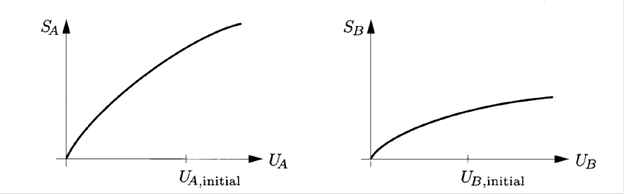
\includegraphics[width=0.9\textwidth]{figs/fig1.png}
    \caption{B has a shallower entropy/energy graph(higher temperature), and the total system will gain entropy if it gives away energy to A.}
\end{figure}

\begin{figure}[H]
    \centering
    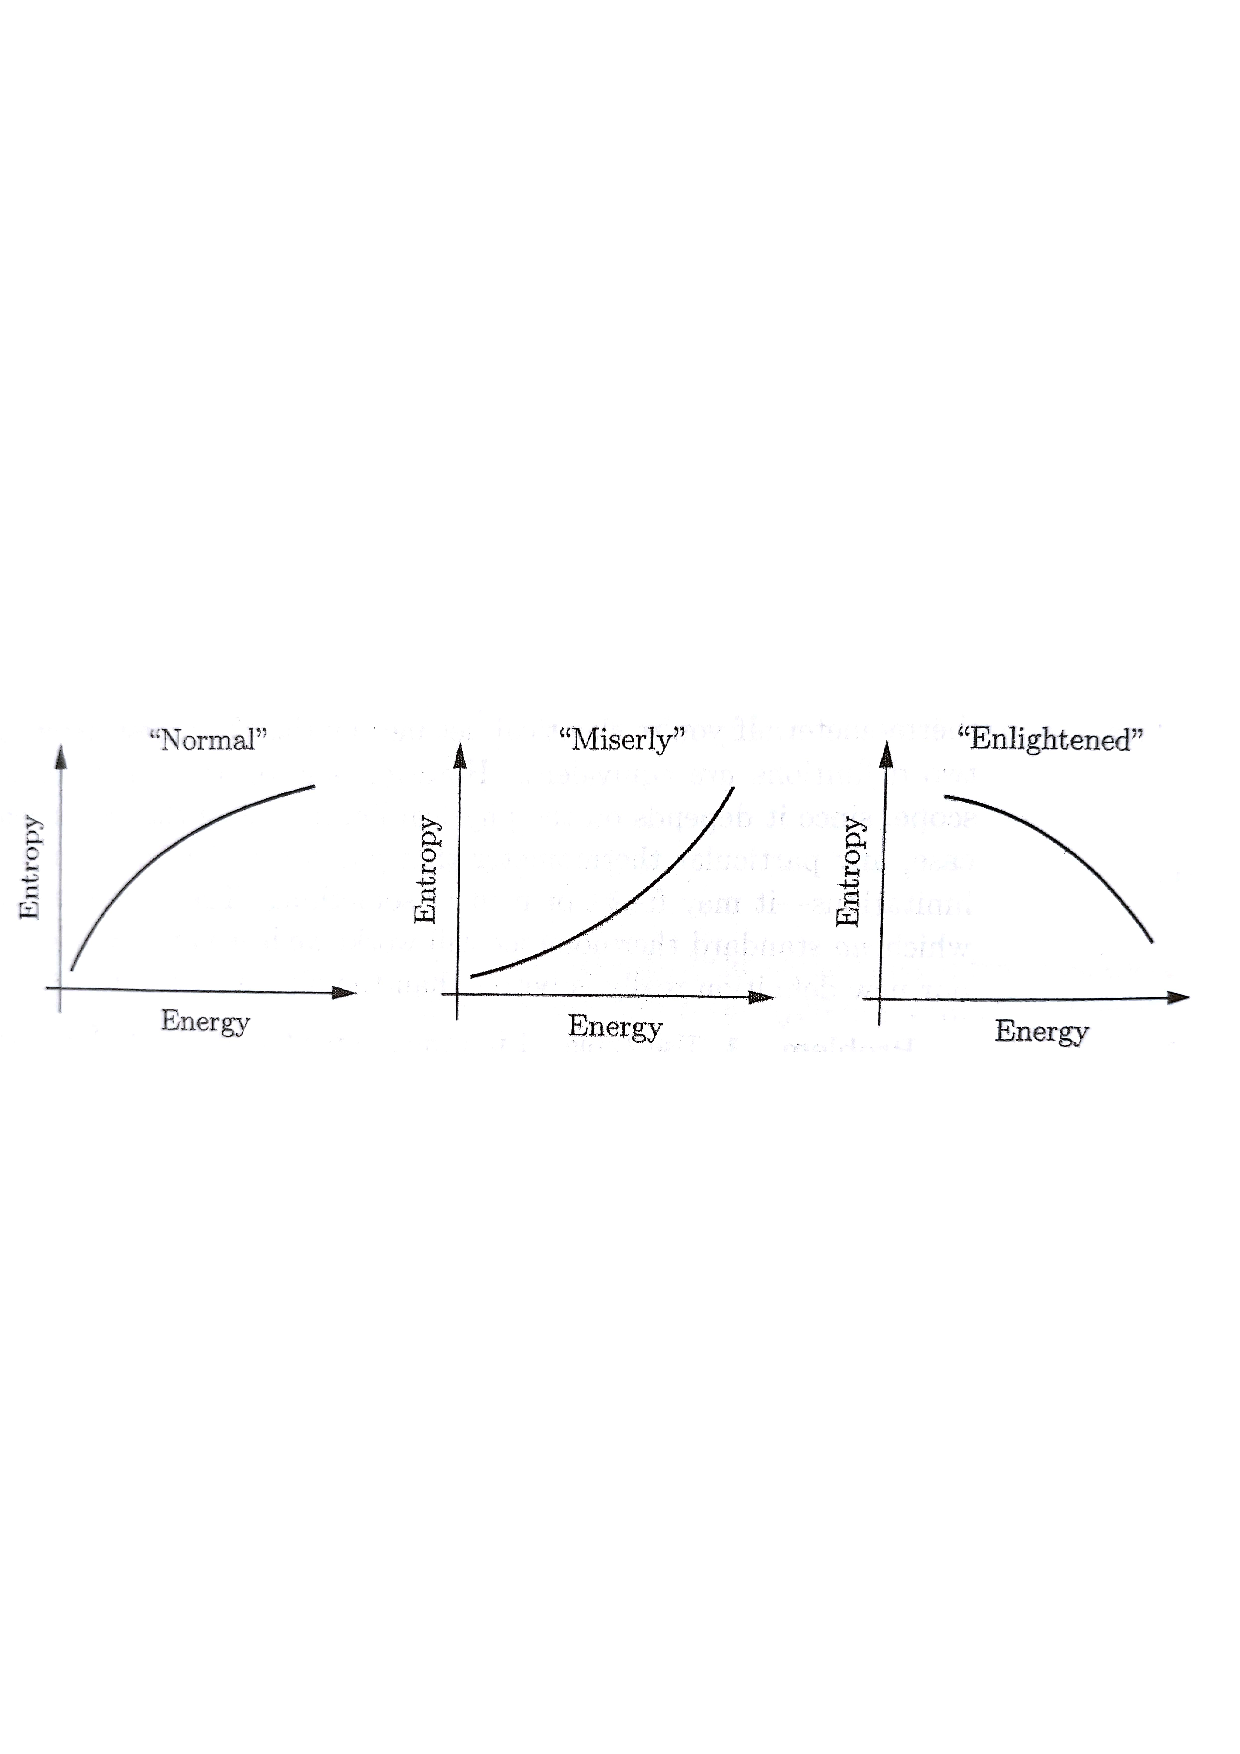
\includegraphics[width=\textwidth, trim={0 12cm 0 12cm}]{figs/fig2.pdf}
    \caption{Systems usually have a logarithmic looking entropy/energy graph, but it might also be exponential, meaning the temperature and willingness to give up energy decreases as it gains more energy. }
\end{figure}
\end{framed}


\rdd{\textbf{Entropy and Heat}}
\begin{framed}
\textbf{Measuring entropy from heat or heat capacity}\\
We can measure the entropy by applying some heat to the system (volume held constant, and no work done). Using the definition of temperature \ref{eqn:T_def}, and applying the definition of heat capacity at constant volume, we can rewrite this as a functions of temperature and heat capacity:
\vspace{-.2cm}\[
	\yl{\dd{S}} = \frac{\dd{S}}{T} = \frac{Q}{T} = 
	\frac{\dd{U}}{T} \yl{= \frac{C_V}{T} \dd{T}}
\]\vspace{-.2cm}

This might seem troublesome when $T \rightarrow 0$. Therefore, we introduce the \bll{\textbf{Third Law of Thermodynamics:}}
\vspace{-.2cm}\[
	C_V \rightarrow 0 \quad \text{as} \quad T \rightarrow 0
\]\vspace{-.2cm}
\end{framed}



\rdd{\textbf{Entropy of a Two-State Paramagnet}}
\begin{framed}
We remember that the two-state paramagnet is a system of $N$ particles, oriented up or down, with or against an external magnetic field. We now introduce the magnetization
\vspace{-.2cm}\[
    M = \mu(N_\uparrow - N_\downarrow) = - \frac{U}{B}
\]
Looking at the multiplicity \ref{eqn:paramag_multi} of the paramagnet, we see that it has its maximum entropy at $N_\uparrow = N_\downarrow \ \rightarrow\ U = 0$

Consider the three regions:
\begin{itemize}
    \item $U < 0,\ N_\uparrow > N_\downarrow$: Positive entropy/energy graph, with positive, and increasing, positive temperature.
    \item $U = 0,\ N_\uparrow = N_\downarrow$: Constant entropy/energy graph, infinite temperature.
    \item $ U > 0,\ N_\uparrow < N_\downarrow$: Negative entropy/energy graph, negative, and increasing temperature.
\end{itemize}

\begin{figure}[H]
    \centering
    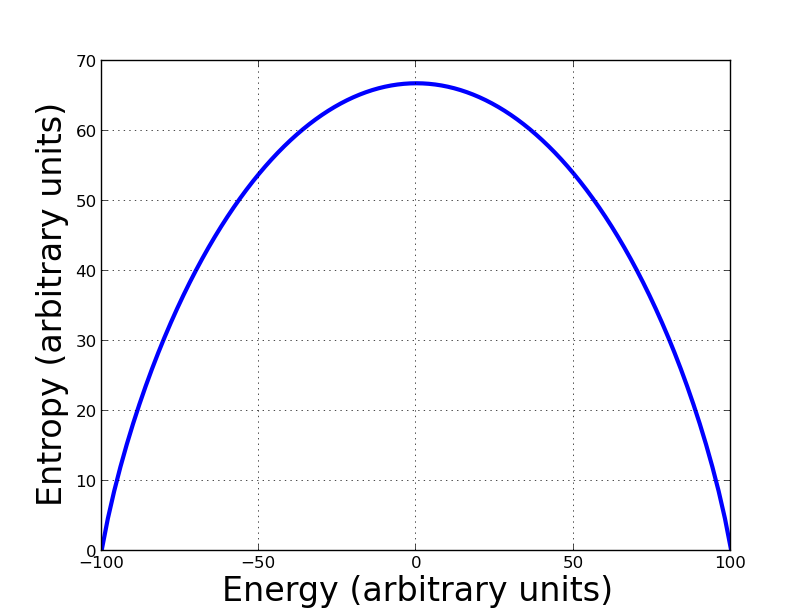
\includegraphics[width=0.49\textwidth]{figs/fig3.png}
    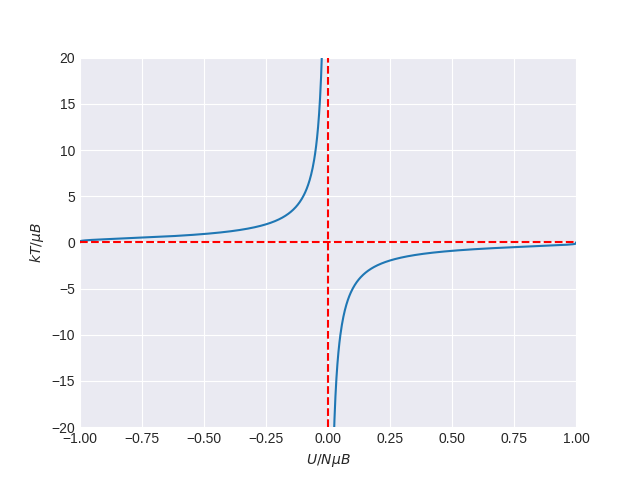
\includegraphics[width=0.49\textwidth]{figs/fig4.png}
    \caption{Entropy/Energy and Temperature/Energy.}
\end{figure}
An infinite temperature system is at its max possible entropy, and will give up energy to any positive temperature system. A negative temperature system will gain entropy by giving away energy, and therefore acts as having "more than infinite" energy.
\end{framed}



\rdd{\textbf{Mechanical Equilibrium and Pressure}}
\begin{framed}
We've looked at the equilibrium state of systems exchanging energy. Now we will look at systems exchanging volume (and indirectly, energy). Corresponding to the temperature definition derived from entropy, we have another for pressure:
\vspace{-.2cm}\begin{align}
    \yl{P = T\qty(\pdv{S}{V})_{U,N}}
\end{align}\vspace{-.2cm}
\end{framed}


\rdd{\textbf{Diffusive Equilibrium and Chemical Potential}}
\begin{framed}
The third type of equilibrium comes from the exchange of particles. \grr{\textbf{Chemical potential}} is the thing that's the same for two systems in \textit{diffusive equilibrium}, meaning that they can gain no more entropy by exchanging particles. A system with larger chemical potential will give up particles to a system with lower chemical potential, increasing the systems total energy.
\vspace{-.2cm}\begin{align}
    \yl{\mu \equiv -T\qty(\pdv{S}{N})_{U,V}} \quad = \qty(\pdv{U}{N})_{S,V}
\end{align}
From the second definition we see that chemical potential has units of energy, and is the change in energy when adding one particles, holding the volume and entropy constant. Since the entropy must remain fixed, you must usually remove energy, and $\mu$ is negative.

Note that everything we talked about slopes of entropy/energy graphs also applies to mechanical and diffusive equilibrium, just with entropy/pressure, and entropy/particles.
\end{framed}


\rdd{The Thermodynamic Identity}
\begin{framed}
Imagine we change a systems entropy by first changing its energy, then volume, then number of particles, each while holding the others fixed. Using the equilibrium identities, we get:
\vspace{-.2cm}\begin{align*}
    \Delta S &= (\Delta S)_{N,V} + (\Delta S)_{N,U} + (\Delta S)_{U,V} \\
             &= \qty(\pdv{S}{U})_{N,V}\dd{U} + \qty(\pdv{S}{V})_{N,U}\dd{V} + \qty(\pdv{S}{N})_{U,V}\dd{N} \\
             &= \frac{1}{T}\dd{U} + \frac{P}{T}\dd{V} - \frac{\mu}{T}\dd{N}
\end{align*}
Rewriting as a function of $\dd{U}$, this becomes\\
\grr{\textbf{The Thermodynamic Identity}}:
\vspace{-.2cm}\begin{align}
    \yl{\dd{U} = T\dd{S} - P\dd{V} + \mu\dd{N}}
\end{align}\vspace{-.2cm}
\end{framed}




%  ██████╗██╗  ██╗ █████╗ ██████╗ ████████╗███████╗██████╗     ███████╗
% ██╔════╝██║  ██║██╔══██╗██╔══██╗╚══██╔══╝██╔════╝██╔══██╗    ██╔════╝
% ██║     ███████║███████║██████╔╝   ██║   █████╗  ██████╔╝    ███████╗
% ██║     ██╔══██║██╔══██║██╔═══╝    ██║   ██╔══╝  ██╔══██╗    ╚════██║
% ╚██████╗██║  ██║██║  ██║██║        ██║   ███████╗██║  ██║    ███████║
%  ╚═════╝╚═╝  ╚═╝╚═╝  ╚═╝╚═╝        ╚═╝   ╚══════╝╚═╝  ╚═╝    ╚══════╝
\section*{\colorbox{red}{*CHAP 5: Free Energy and Chemical Thermodyn.*}}
\rdd{\textbf{The Thermodynamic Potentials}}
\begin{framed}
\begin{align*}
    \text{(Enthalpy)} \quad &\yl{H \equiv U + PV} &\dd{H} = \dd{U} + V\dd{P} + P\dd{V}\\
    \text{(Helmholtz Free Energy)} \quad &\yl{F \equiv U - TS} &\dd{F} = \dd{U} - S\dd{T} - T\dd{S} \\
    \text{(Gibbs Free Energy)} \quad &\yl{G \equiv U - TS + PV} &\dd{G} = \dd{F} + P\dd{V} + V\dd{P} \\
    & = F + PV = H - TS
\end{align*}\vspace{-.4cm}

Enthalpy = Energy of system + energy to make room for it.\\
Helmholtz = Energy of system - energy we can lend from reservoar at temp $T$.\\
Gibbs = The two above combined.

Remembert that tese are linear in $U$, so any increase in $U$ is a direct increase in all.

By inserting the thermodynamic identity for $\dd{U}$, we derive the thermodynamic identities for each potential:
\vspace{-.2cm}\begin{align*}
    &\yl{\dd{H}\: = T\dd{S} + V\dd{P} + \mu\dd{N}} \\
    &\yl{\dd{F} = -S\dd{T} - P\dd{V} + \mu\dd{N}} \\
    &\yl{\dd{G} = -S\dd{T} + V\dd{P} + \mu\dd{N}}
\end{align*}
Setting some of these parameters constant, we can derive:
\vspace{-.2cm}\[
    S = -\qty(\pdv{F}{T})_{V,N} \quad
    P = -\qty(\pdv{F}{V})_{T,N} \quad
    \mu = \qty(\pdv{F}{N})_{T,V}
\]
\vspace{-.2cm}\[
    S = -\qty(\pdv{G}{T})_{P,N} \quad
    V = -\qty(\pdv{G}{P})_{T,N} \quad
    \mu = \qty(\pdv{G}{N})_{T,P}
\]\vspace{-.2cm}

By switching the order of derivations, and setting them equal, we get the \bll{\textbf{Maxwell Relations}}:
\begin{align*}
	\pdv[2]{U}{S}{V} = \yl{\qty(\pdv{T}{V})_S = - \qty(\pdv{P}{S})_V} \quad\quad
	&\pdv[2]{H}{S}{P} = \yl{\qty(\pdv{V}{S})_P = \qty(\pdv{T}{P})_S} \\
	-\pdv[2]{F}{T}{V} = \yl{\qty(\pdv{P}{T})_V = \qty(\pdv{S}{V})_T} \quad\quad
	&\pdv[2]{G}{T}{P} = \yl{\qty(\pdv{V}{T})_P = - \qty(\pdv{S}{P})_T}
\end{align*}\vspace{-.4cm}

\begin{tcolorbox}[title={Validity},top=0cm,bottom=0cm,right=0.1cm,left=0.1cm]
    When dealing with all these derivatives, the subscripts indicate what parameters are to be held constant during the derivation. We are not allowed to use an identitiy of one of these values depend on the derivative. For example, if $V$ is a function of $N$, but $P$ is not, we can use $\mu = \qty(\pdv{G}{N})_{T,P}$, but not $\mu = \qty(\pdv{F}{N})_{T,V}$.
\end{tcolorbox}

We also have the very usefull relation \yll{$G = \mu N$}.
\end{framed}



\rdd{\textbf{Free Energy as a Force toward Equilibrium}}
\begin{framed}
Systems in contact with some reservoar is often of interest. Here, we can't use the 2. law on the system, because it's the entropy of the system + the enviroment that tends to increase. It turns out that
\begin{itemize}
    \item \grr{At constant energy and volume, $S$ tends to increase.}
    \item \grr{At constant temperature and volume, $F$ tends to decrease.} This happens when we can exchange temperature with a reservoar, but the volume is held constant.
    \item \grr{At constant temperature and pressure, $G$ tends to decrease.} This happens when our volume can change, and we are held at the same pressure as the reservoar.
\end{itemize}
we can do the assumptions that these values are then at their minimum in a equilibrium system.


\textbf{Extensive and Intensive Quantities}\\
Extensive properties double when we double the size of the system, while intensive properties stay the same.
\begin{itemize}
    \item Extensive: $V$, $N$, $S$, $U$, $H$, $F$, $G$, mass
    \item Intensive: $T$, $P$, $\mu$, density
\end{itemize}
Multiplying an intensive and extensive property creates an extensive one. Multiplying two extensive is undefined, and might be an error.
\end{framed}



\rdd{\textbf{Phase Transformations}}

\begin{wrapfigure}{R}{0.33\textwidth}
    \centering
    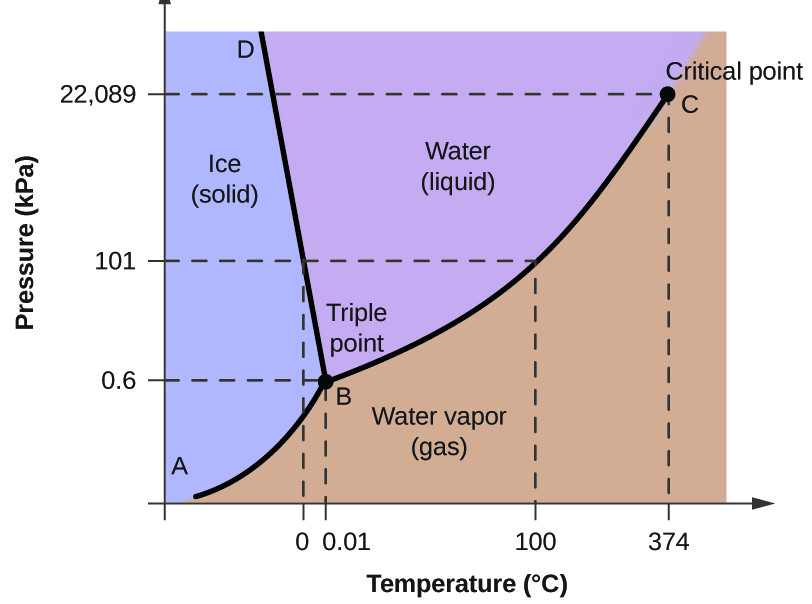
\includegraphics[width=0.33\textwidth]{figs/fig5.jpg}
\end{wrapfigure}

A phase transformation is a discontinious change in a substance properties from an infinitesimal change in its enviroment. This is usually a function of \textit{pressure}, and \textit{temperature}.

Gibbs free energy is the paramter of interest, as the system will attempt to minimize it. The most stable element will be the one with the lowest $G$.

\bll{\textbf{Damptrykk:}} Pressure where phase transformation takes place. In the equilibrium between two phases, \grr{their gibbs factors and chemical potentials are the same:} $\mu_g = \mu_l$, $G_g = G_l$.
\\
\\
\rdd{\textbf{Clausius-Clapeyron modellen}}
Entropi bestemmer temperaturavhengigheten til Gibbs, og volum bestemmer trykkavhengigheten (se identitier ved potensialene). At a phase boundry, both gas and liquid will be stable, and we have $G_g = G_l$, inserting the thermodynamic relations gives
$\dv{P}{T} = \frac{S_g - S_l}{V_g - V_l} = \frac{L}{T\Delta V}$ (remember that $V_g \gg V_l$).


\rdd{\textbf{Wan der Waal Model}}
Approxtion model for atomic interaction forces:
$$
    \qty(P + \frac{aN^2}{V^2})\qty(V - Nb) = NkT
$$



%  ██████╗██╗  ██╗ █████╗ ██████╗ ████████╗███████╗██████╗      ██████╗ 
% ██╔════╝██║  ██║██╔══██╗██╔══██╗╚══██╔══╝██╔════╝██╔══██╗    ██╔════╝ 
% ██║     ███████║███████║██████╔╝   ██║   █████╗  ██████╔╝    ███████╗ 
% ██║     ██╔══██║██╔══██║██╔═══╝    ██║   ██╔══╝  ██╔══██╗    ██╔═══██╗
% ╚██████╗██║  ██║██║  ██║██║        ██║   ███████╗██║  ██║    ╚██████╔╝
%  ╚═════╝╚═╝  ╚═╝╚═╝  ╚═╝╚═╝        ╚═╝   ╚══════╝╚═╝  ╚═╝     ╚═════╝
\section*{\colorbox{red}{*******CHAPTER 6: Boltzmann Statistics*******}}
As we have already seen, we often wish to explore a system in contact with an enviroment. We can then not directly use neither the 2. law, or the assumption that every microstate is equally probable, because these are the entropies and microstates of the system \textit{and} the enviroment.

We will now instead delevop a powerful tool for calculating the probability of microstates in a non-isolated system in thermal contact with a reservoar.

\rdd{\textbf{The Boltzmann Factor}}
\begin{framed}
The Boltzmann Factor of a microstate $s$, is the \textit{relative} probability of finding the system in that microstate, as a function of its energy and temperature:
\vspace{-.2cm}\begin{align}
    \text{Boltzmann Factor}= \exp{-E(s)/kT}
\end{align}
The absolute probability will then come from normalizing the Boltzmann Factor:
\vspace{-.2cm}\[
    \mathcal{P}(s) = \frac{1}{Z} \exp{-E(s)/kT}
\]\vspace{-.2cm}
where the \grr{\textbf{Partition Function}} $Z$ is the sum of all possible states:
\vspace{-.2cm}\begin{align}
    Z = \sum\limits_{s} \exp{-E(s)/kT}
\end{align}
This statement is very powerful, requiring only knowledge of the energy of every state to calculate every probability.

\bll{DEF - Degeneracy:} When an energy level corresponds to more than one microstate, it is called degenerate. When calculating the probability of that energy, we must multiply by the number of microstates with that energy.
\end{framed}


\rdd{\textbf{Average Values}}
\begin{framed}
First, let's introduce a shorthand notation:
$   
    \yl{\beta = 1/kT}
$\\
Calculating expectation values (average values) are done the usual way, since the probability distribution is known. For a property $X(s)$, we have the expectation value
$
    \yl{\bar{X} =} \sum\limits_s X(s)\mathcal{P}(s) = \yl{\frac{1}{Z} \sum\limits_s X(s) \exp{-\beta E(s)}}
$\\
It can be shown that for the energy, this average becomes
\vspace{-.2cm}\[
    \yl{\bar{E} = -\frac{1}{Z}\pdv{Z}{\beta}} = -\pdv{\beta} \ln{Z}
\]\vspace{-.2cm}
\end{framed}



\rdd{\textbf{The Equipartition Theorem}}
\begin{framed}
The equipartition theorem has been a useful tool. Turns out it's provable with Boltzmann factors. The proof is however dependent on the assumption that the spacing between energy levels is somewhat continious (much less than $kT$). This mean \textbf{the equipartition theorem can not be used in quantum mechanics.}
\end{framed}

\textbf{Maxwell Speed Distribution}\\



\rdd{\textbf{Partition Functions and Free Energy}}
\begin{framed}
\begin{table}[H]
	\centering
	\begin{tabular}{ M{2.4cm} | M{2.4cm} M{2.4cm} }
		System Type     & Isolated           &  Contact with reservoar \\
		\hline
		\vspace{0.2cm}Fixed Parameter & \vspace{0.2cm} \ \ \ Energy\newline($U$)       &  \vspace{0.2cm}Temperature\newline ($T$) \\
		\vspace{0.2cm}Governing Property &\vspace{0.2cm} \ \ Multiplicity\newline ($\Omega$) & \vspace{0.2cm} Partition \newline Function\newline ($Z$) \\
		\vspace{0.2cm}Tendency        &\vspace{0.2cm} $S = k\ln{\Omega}$\newline (increases) &\vspace{0.2cm}  $F = -kT\ln{Z}$\newline (decreases)
	\end{tabular}
\end{table}\vspace{-0.4cm}

As we can see from the table above, the partition function ($Z$) plays some of the same role in a non-isolated system as the the multiplicity ($\Omega$) does in an isolated system, telling us something about the total amount of avaliable microstates. We can also establish a similar definition to the entropy/multiplicity one, using the Helmholtz Energy, which is the parameter destined to decrease in a non-isolated system:
$
    \yl{F = -kT\ln{Z}} \quad \text{or} \quad \yl{Z = \exp{-F/kT}}
$\\
Looking back at section 5.1, we can see that if we know the partition function of a system, we know all its thermodynamic properties, since they can be calculated from the Helmholtz energy.
\end{framed}



\rdd{\textbf{Partition Function for Composite Systems}}
\begin{framed}
A nice property the partition function shares with multiplicity is that it's ususally multiplicable, due to basic combinatorics

If we look at a system of several, non-interacting, distinguishable particles, the total partition function is merely the product of the individuals:
\vspace{-.2cm}\[
    Z_\text{total} = Z_1Z_2...Z_N \quad \text{(noninteracting, distinguishable)}
\]
If however the particles are identical, we have overcounted a lot of the states, as interchanging two particles yields the same state. The partition functions of the particles must also be identical if they are identical, and the total partition function becomes:
\vspace{-.2cm}\[
    \yl{Z_\text{total} = \frac{1}{N!}Z_1^N} \quad \text{(noninteracting, indistinguishable)}
\]
The factor $N!$ is actually slightly too high, as some of the states in $Z$ involves some of the particles in the same state, meaning they weren't double-counted in the first place. This is however not a big problem as long as the system isn't too dense.
\end{framed}



\rdd{\textbf{Ideal Gas Revised}}
\begin{framed}
We decompose the partition function into a "translatoric energy" and "internal energy"(like atomic bonds) parts: $Z = Z_\text{tr}Z_\text{int}$. 

The allowed energies of a single ideal gas particle in a box of size $L$ are, according to Q.M:
\vspace{-.2cm}\[
    E_n = \frac{h^2n^2}{8mL^2} \ , \ \ n\in\{1,2,3...\}
\]\vspace{-.2cm}
giving a partition function (in 1 dimension):
\vspace{-.2cm}\[
    \yl{Z_\text{tr, 1D} =} \sum\limits_n \exp{-h^2n^2/8mL^2kT} \approx \int\limits_0^\infty \exp{-h^2...}\dd{n} = \yl{\frac{L}{l_Q}}
\]\vspace{-.2cm}
where
\vspace{-.2cm}\[
    l_Q \equiv \frac{h}{\sqrt{2\pi m k T}}
\]
is the \textbf{quantum length}, which is just the de Broglie length scaled by $\pi$. Upscaling to 3 dimensions gives
$
    \yl{Z_\text{tr, 3D} = \frac{V}{v_Q}} = \frac{L_x L_y L_z}{l_Q^3}
$
Combining this with the internal partition function gives $Z_1 = \frac{V}{v_Q}Z_\text{int}$, which for a system of $N$ indistinguishable particles becomes
$
    \yl{Z = \frac{1}{N!}\qty(\frac{V Z_\text{int}}{v_Q})^N}
$

\textbf{Energy:} $U = -\pdv{Z}{\beta} = \frac{3}{2}NkT$ \ \ \ \ \ 
\textbf{Entropy:} $S = \frac{U - F}{T} = Nk\qty[\ln{\frac{V}{Nl_Q}} + \frac{5}{2}]$
\end{framed}


\rdd{\textbf{Maxwell Speed Distribution}}
\begin{framed}
Distribution function of ideal gas velocities should be proportional to \textit{probability that particle has speed$\b v$ ($4\pi v^2$)} times \textit{number of vectors corresponding to speed $v$, $4\pi v^2$}, giving $\mathcal{D}(v) \propto \qty(\exp{-mv^2/2kT})\times \qty(4\pi v^2)$. Normalizing the integral over it to $1$ gives
$\mathcal{D}(v) = \qty(\frac{m}{2\pi kT})^{3/2}4\pi v^2 \exp{-mv^2/2kT}$.
\end{framed}



%  ██████╗██╗  ██╗ █████╗ ██████╗ ████████╗███████╗██████╗     ███████╗
% ██╔════╝██║  ██║██╔══██╗██╔══██╗╚══██╔══╝██╔════╝██╔══██╗    ╚════██║
% ██║     ███████║███████║██████╔╝   ██║   █████╗  ██████╔╝        ██╔╝
% ██║     ██╔══██║██╔══██║██╔═══╝    ██║   ██╔══╝  ██╔══██╗       ██╔╝ 
% ╚██████╗██║  ██║██║  ██║██║        ██║   ███████╗██║  ██║       ██║  
%  ╚═════╝╚═╝  ╚═╝╚═╝  ╚═╝╚═╝        ╚═╝   ╚══════╝╚═╝  ╚═╝       ╚═╝
\section*{\colorbox{red}{*******CHAPTER 7: Quantum Statistics*******}}
\bll{DEF - System State:} An unique configuration of the entire system. \\
\bll{DEF - State:} Single particle state (i.e. "in this specific energy level").



\rdd{\textbf{The Gibbs Factor}}
\begin{framed}
Boltzmann statistics was built on the change in entropy when a system goes from a state $1$ to $2$. Let's do the same, but allow the exchange of particles between the system and reservoar, giving us the \grr{\textbf{Gibbs Factor:}}
\vspace{-.2cm}\begin{align}
    \text{Gibbs factor}= \exp{-[E(s)-\mu N(s)]/kT}
\end{align}
which is the equivalent of the Boltzmann factor when exchange of particles is allowed. In other words, it is the relative probability of finding the system in a state $s$. It is also derived from the thermodynamic identity, \textit{assuming $P\dd{V}$ to be negligible}.

With it comes a normalization factor called the\\ \grr{\textbf{Grand Partition Function:}}
$
    \yl{\mathcal{Z} = \sum\limits_s \exp{-[E(s)-\mu N(s)]/kT}}
$
\end{framed}


\rdd{\textbf{Bosons and Fermions}}
\begin{framed}
In a high-density system where two particles are likely to compete for the same state,the total number of system states depend alot on whether two particles are allowed to occupy the same state. This depends on what kind of particles we are dealing with:
\begin{itemize}
    \item \grr{\textbf{Bosons:}} Multiple bosons can share the same state.
    \item \grr{\textbf{Fermions:}} Only one fermion can occupy one state.
\end{itemize}
The force keeping fermions from occupying the same state is called the \grr{\textbf{Pauli Exclusion Principle}}. The principle is, however, only relevant where the density is high enough that two particles are actually likely to occupy the same state. In other words, the total number of avaliable states are in the same order of magnitude as the number of particles. If not we have the \bll{\textbf{Classical Limit:}}
$
    \yl{Z_1 \gg N}
$\\
For an ideal gas, this would be
$
    \yl{\frac{V}{N} \gg v_Q} \quad \text{(Classical limit, ideal gas)}
$\\
which results in $(\epsilon - \mu)/kT \gg 1$.
\end{framed}

\rdd{\textbf{The Distribution Function}}
\begin{framed}
We will start with an intuition struggle. Imagine that the "system" is simply one possible single particle state (like an energy level in an harmonic oscilator), and that the reservoar is all other possible single particle states (other energy levels). Since the system is free to recieve and give away particles at will, we will need Gibbs, not Boltzmann for this one. If the state's energy is $\epsilon$, the probability that the state is occupied by $n$ particles (considered we're talking about bosons) is
\vspace{-.2cm}\[
    \mathcal{P}(n) = \frac{1}{\mathcal{Z}}\exp{-n(\epsilon - \mu)/kT}
\]
\textbf{Fermions}\\
If we're talking about fermions, $n$ can only be $0$ or $1$, and the Grand Parition Function becomes
\vspace{-.2cm}\[
    \mathcal{Z} = 1 + \exp{-(\epsilon-\mu)/kT}
\]
and the probability that the state is occupied by the one possible particle is
\vspace{-.2cm}\[
    \yl{\bar{n}_\text{FD} = \frac{1}{\exp{(\epsilon- \mu)/kT} + 1}} \quad \text{(Fermion occupancy)}
\]
This is called the \grr{\textbf{Fermi-Diraq Distribution}}, and decides the probability that a state is occupied (for fermions).

\textbf{Bosons}\\
For bosons, the Grand Parition Function becomes
\vspace{-.2cm}\[
    \mathcal{Z} = 1 + \exp{-(\epsilon - \mu)/kT} + \exp{-2(\epsilon - \mu)/kT} + ... = \frac{1}{1 - \exp{-(\epsilon-\mu)/kT}}
    \]
giving (after som calculation)
\vspace{-.2cm}\[
    \yl{\bar{n}_\text{BE} = \frac{1}{\exp{(\epsilon - \mu)/kt} - 1}} \quad \text{(Boson occupancy)}
\]\vspace{-.1cm}
and is called the \grr{\textbf{Bose-Einstein Distribution}}

Both these distribution approach the Boltzmann Distribution in the high-energy classical limit, $\epsilon \gg kT$
\end{framed}


\rdd{\textbf{Degenerate Fermi Gasses}}
\begin{framed}
\bll{DEF - Degeneracy:} Degenerate has a second definition, describing cases where there is a very hard limit between occupied an unoccupied states.

\bll{\textbf{Density of States:}} $D(\epsilon)$ or $D(n)$ represents the density of avaliable states at an energy $\epsilon$ or number $n=\sqrt{n_x^2 + n_y^2 + n_z^2}$, in such a way that\\
$N = \int_0^{\epsilon_F} D(\epsilon) \dd{\epsilon}$ is the total number of avaliable states up to $\epsilon_F$ (or a number $n$).\quad\quad\quad\quad DoS:(Including 2 spin states)\\
1D: $D(n) = 2$\\
2D: $D(n) = 2\cdot \frac{1}{4}\cdot 2\pi n_\text{max} = \pi n_\text{max}$\\
3D: $D(n) = 2\cdot \frac{1}{8}\cdot 4 \pi n_\text{max}^2 = \pi n_\text{max}^2$

\vspace{-.3cm}\[
    \yl{D(n) \dd{n} = D(\epsilon) \dd{\epsilon}}
\]\vspace{-.2cm}

\bll{\textbf{Zero Temperature}}\\
In the zero-temperature case, the particles simply fill up the lowest possible energy states, up to a hard limit
$    \yl{\epsilon_F \equiv \mu(T = 0)} \quad \text{(Fermi Energy)}
$
and the Fermi-Dirac funtion becomes a step-function. 

The allowed energy levels of a particle in a box is know from Q.M. as (in 3D):
\vspace{-.2cm}\[
    \epsilon = \frac{h^2}{8mL^2}(n_x^2 + n_y^2 + n_z^2) \ , \ \ n \in \{1,2,3...\}
\]
Instead of a "step-function" this becomes a quarter-sphere with surface $n_x^2 + n_y^2 + n_z^2 = n_\text{max}^2$, corresponding to the fermi energy:
$    \epsilon_F = \frac{h^2n_\text{max}^2}{8mL^2}
$

The number of such states enclosed is equivalent to the volume of this quarter-sphere (times 2 from spins)
\vspace{-.2cm}\[
    N = 2\cdot\frac{1}{8}\cdot \frac{4}{3}\pi n_\text{max}^3 = \frac{\pi n_\text{max}^3}{3}
\]\vspace{-.2cm}
giving the fermi-energy
\vspace{-.2cm}\[
    \epsilon_F = \frac{h^2}{8m}\qty(\frac{3N}{\pi V})^{2/3}
\]\vspace{-.2cm}
Energy inside fermi surface:
\begin{align*}
    U = 2 \sum_{n_x}\sum_{n_y}\sum_{n_z} \epsilon(\vec{n}) = 2\cdot\int\int\int \epsilon(\vec{n})\dd{n_x}\dd{n_y}\dd{n_z} =\\
    = 2\int_0^{n_{max}}\int_0^{\pi/2}\int_0^{\pi/2}\epsilon(n)\dd{\phi}\dd{\theta}\dd{n} 
    = \pi\int_0^{n_\text{max}}\epsilon(n)n^2\sin{\theta} \dd{n} = \frac{3}{5}N \epsilon_F
\end{align*}


\bll{\textbf{Small, non-zero Temperatures}}
In the non-zero case, we need to multiply the density of states with the probability that the state is occupied:
\[
    N = \int_0^\infty D(\epsilon)\cdot \bar{n}_\text{FD}(\epsilon) \dd{\epsilon} = \int_0^\infty \frac{D(\epsilon)}{\exp{(\epsilon-\mu)/kT} + 1} \dd{\epsilon} \quad\ (T \neq 0)
\]
\[
    U = \int_0^\infty\epsilon \cdot D(\epsilon)\cdot \bar{n}_\text{FD}(\epsilon) \dd{\epsilon} = \int_0^\infty \frac{\epsilon\cdot D(\epsilon)}{\exp{(\epsilon-\mu)/kT} + 1} \dd{\epsilon} \quad\ (T \neq 0)
\]

\bll{\textbf{Classical Limit:}} $Z_1 \gg N \quad \Rightarrow \quad \mu \ll  kT$
\end{framed}

\bll{\textbf{Blackbody Rad:}}$Z = 1 + \exp{-\beta h f} + \exp{-2\beta h f} + \cdots = \frac{1}{1-\exp{-\beta h f}}$.\\
Plack Dist (Avg Eng): $\bar{E} = \frac{1}{Z}\pdv{Z}{\beta} = \frac{hf}{\exp{hf/kT} - 1}$.\\
$\mu_e = \mu_e + \mu_gamma \quad\Rightarrow\quad \mu = 0$ for photons.\\
Etropy of photon gas: $C_V = \pd{U}{V}{T} 4aT^3$, $S(T) = \int_0^T\frac{C_V(T')}{T'}\dd{T'} = \frac{32\pi^5Vk}{45}(\frac{kT}{hv})^3$.

\end{twocolumn}
\end{document}
